\documentclass{extbook}[14pt]
\usepackage{multicol, enumerate, enumitem, hyperref, color, soul, setspace, parskip, fancyhdr, amssymb, amsthm, amsmath, bbm, latexsym, units, mathtools}
\everymath{\displaystyle}
\usepackage[headsep=0.5cm,headheight=0cm, left=1 in,right= 1 in,top= 1 in,bottom= 1 in]{geometry}
\usepackage{dashrule}  % Package to use the command below to create lines between items
\newcommand{\litem}[1]{\item #1

\rule{\textwidth}{0.4pt}}
\pagestyle{fancy}
\lhead{}
\chead{Answer Key for Makeup Progress Quiz 3 Version B}
\rhead{}
\lfoot{4315-3397}
\cfoot{}
\rfoot{Fall 2020}
\begin{document}
\textbf{This key should allow you to understand why you choose the option you did (beyond just getting a question right or wrong). \href{https://xronos.clas.ufl.edu/mac1105spring2020/courseDescriptionAndMisc/Exams/LearningFromResults}{More instructions on how to use this key can be found here}.}

\textbf{If you have a suggestion to make the keys better, \href{https://forms.gle/CZkbZmPbC9XALEE88}{please fill out the short survey here}.}

\textit{Note: This key is auto-generated and may contain issues and/or errors. The keys are reviewed after each exam to ensure grading is done accurately. If there are issues (like duplicate options), they are noted in the offline gradebook. The keys are a work-in-progress to give students as many resources to improve as possible.}

\rule{\textwidth}{0.4pt}

\begin{enumerate}\litem{
Construct the lowest-degree polynomial given the zeros below. Then, choose the intervals that contain the coefficients of the polynomial in the form $ax^3+bx^2+cx+d$.
\[ -1, -6, \text{ and } \frac{5}{2} \]

The solution is \( 2x^{3} +9 x^{2} -23 x -30 \), which is option A.\begin{enumerate}[label=\Alph*.]
\item \( a \in [1, 4], b \in [8, 10.2], c \in [-27, -22], \text{ and } d \in [-36, -26] \)

* $2x^{3} +9 x^{2} -23 x -30$, which is the correct option.
\item \( a \in [1, 4], b \in [8, 10.2], c \in [-27, -22], \text{ and } d \in [23, 31] \)

$2x^{3} +9 x^{2} -23 x + 30$, which corresponds to multiplying everything correctly except the constant term.
\item \( a \in [1, 4], b \in [-19.9, -15.6], c \in [42, 56], \text{ and } d \in [-36, -26] \)

$2x^{3} -19 x^{2} +47 x -30$, which corresponds to multiplying out $(x -1)(x -6)(2x -5)$.
\item \( a \in [1, 4], b \in [-12.1, -5.2], c \in [-27, -22], \text{ and } d \in [23, 31] \)

$2x^{3} -9 x^{2} -23 x + 30$, which corresponds to multiplying out $(x -1)(x -6)(2x + 5)$.
\item \( a \in [1, 4], b \in [4.5, 8.8], c \in [-39, -32], \text{ and } d \in [23, 31] \)

$2x^{3} +5 x^{2} -37 x + 30$, which corresponds to multiplying out $(x -1)(x + 6)(2x -5)$.
\end{enumerate}

\textbf{General Comment:} To construct the lowest-degree polynomial, you want to multiply out $(x + 1)(x + 6)(2x -5)$
}
\litem{
Construct the lowest-degree polynomial given the zeros below. Then, choose the intervals that contain the coefficients of the polynomial in the form $x^3+bx^2+cx+d$.
\[ 4 + 3 i \text{ and } -2 \]

The solution is \( x^{3} -6 x^{2} +9 x + 50 \), which is option C.\begin{enumerate}[label=\Alph*.]
\item \( b \in [5, 17], c \in [6, 9.1], \text{ and } d \in [-53.4, -49.1] \)

$x^{3} +6 x^{2} +9 x -50$, which corresponds to multiplying out $(x-(4 + 3 i))(x-(4 - 3 i))(x -2)$.
\item \( b \in [0, 4], c \in [-3.7, -1.4], \text{ and } d \in [-11, -7.5] \)

$x^{3} + x^{2} -2 x -8$, which corresponds to multiplying out $(x -4)(x + 2)$.
\item \( b \in [-14, 0], c \in [6, 9.1], \text{ and } d \in [49.6, 50.9] \)

* $x^{3} -6 x^{2} +9 x + 50$, which is the correct option.
\item \( b \in [0, 4], c \in [-1.8, 0.5], \text{ and } d \in [-6.5, -1.6] \)

$x^{3} + x^{2} -x -6$, which corresponds to multiplying out $(x -3)(x + 2)$.
\item \( \text{None of the above.} \)

This corresponds to making an unanticipated error or not understanding how to use nonreal complex numbers to create the lowest-degree polynomial. If you chose this and are not sure what you did wrong, please contact the coordinator for help.
\end{enumerate}

\textbf{General Comment:} Remember that the conjugate of $a+bi$ is $a-bi$. Since these zeros always come in pairs, we need to multiply out $(x-(4 + 3 i))(x-(4 - 3 i))(x-(-2))$.
}
\litem{
Construct the lowest-degree polynomial given the zeros below. Then, choose the intervals that contain the coefficients of the polynomial in the form $x^3+bx^2+cx+d$.
\[ -5 + 3 i \text{ and } -1 \]

The solution is \( x^{3} +11 x^{2} +44 x + 34 \), which is option C.\begin{enumerate}[label=\Alph*.]
\item \( b \in [-9, 7], c \in [-3, 0], \text{ and } d \in [-5, 0] \)

$x^{3} + x^{2} -2 x -3$, which corresponds to multiplying out $(x -3)(x + 1)$.
\item \( b \in [-9, 7], c \in [0, 12], \text{ and } d \in [1, 7] \)

$x^{3} + x^{2} +6 x + 5$, which corresponds to multiplying out $(x + 5)(x + 1)$.
\item \( b \in [8, 18], c \in [40, 48], \text{ and } d \in [32, 38] \)

* $x^{3} +11 x^{2} +44 x + 34$, which is the correct option.
\item \( b \in [-13, -7], c \in [40, 48], \text{ and } d \in [-34, -25] \)

$x^{3} -11 x^{2} +44 x -34$, which corresponds to multiplying out $(x-(-5 + 3 i))(x-(-5 - 3 i))(x -1)$.
\item \( \text{None of the above.} \)

This corresponds to making an unanticipated error or not understanding how to use nonreal complex numbers to create the lowest-degree polynomial. If you chose this and are not sure what you did wrong, please contact the coordinator for help.
\end{enumerate}

\textbf{General Comment:} Remember that the conjugate of $a+bi$ is $a-bi$. Since these zeros always come in pairs, we need to multiply out $(x-(-5 + 3 i))(x-(-5 - 3 i))(x-(-1))$.
}
\litem{
Construct the lowest-degree polynomial given the zeros below. Then, choose the intervals that contain the coefficients of the polynomial in the form $ax^3+bx^2+cx+d$.
\[ 3, \frac{5}{2}, \text{ and } \frac{3}{5} \]

The solution is \( 10x^{3} -61 x^{2} +108 x -45 \), which is option D.\begin{enumerate}[label=\Alph*.]
\item \( a \in [6, 17], b \in [61, 69], c \in [102, 110], \text{ and } d \in [44, 50] \)

$10x^{3} +61 x^{2} +108 x + 45$, which corresponds to multiplying out $(x + 3)(2x + 5)(5x + 3)$.
\item \( a \in [6, 17], b \in [-3, 3], c \in [-79, -76], \text{ and } d \in [44, 50] \)

$10x^{3} -1 x^{2} -78 x + 45$, which corresponds to multiplying out $(x + 3)(2x -5)(5x -3)$.
\item \( a \in [6, 17], b \in [46, 56], c \in [41, 44], \text{ and } d \in [-48, -41] \)

$10x^{3} +49 x^{2} +42 x -45$, which corresponds to multiplying out $(x + 3)(2x + 5)(5x -3)$.
\item \( a \in [6, 17], b \in [-61, -59], c \in [102, 110], \text{ and } d \in [-48, -41] \)

* $10x^{3} -61 x^{2} +108 x -45$, which is the correct option.
\item \( a \in [6, 17], b \in [-61, -59], c \in [102, 110], \text{ and } d \in [44, 50] \)

$10x^{3} -61 x^{2} +108 x + 45$, which corresponds to multiplying everything correctly except the constant term.
\end{enumerate}

\textbf{General Comment:} To construct the lowest-degree polynomial, you want to multiply out $(x -3)(2x -5)(5x -3)$
}
\litem{
Describe the zero behavior of the zero $x = -5$ of the polynomial below.
\[ f(x) = 7(x + 7)^{11}(x - 7)^{8}(x + 5)^{3}(x - 5)^{2} \]

The solution is the graph below, which is option D.
\begin{center}
    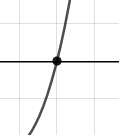
\includegraphics[width=0.3\textwidth]{../Figures/polyZeroBehaviorDB.png}
\end{center}\begin{enumerate}[label=\Alph*.]
\begin{multicols}{2}
\item 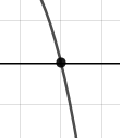
\includegraphics[width = 0.3\textwidth]{../Figures/polyZeroBehaviorAB.png}
\item 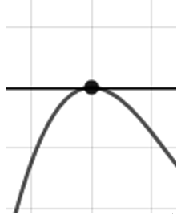
\includegraphics[width = 0.3\textwidth]{../Figures/polyZeroBehaviorBB.png}
\item 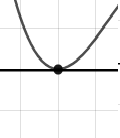
\includegraphics[width = 0.3\textwidth]{../Figures/polyZeroBehaviorCB.png}
\item 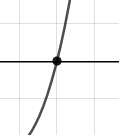
\includegraphics[width = 0.3\textwidth]{../Figures/polyZeroBehaviorDB.png}
\end{multicols}\item None of the above.\end{enumerate}
\textbf{General Comment:} You will need to sketch the entire graph, then zoom in on the zero the question asks about.
}
\litem{
Which of the following equations \textit{could} be of the graph presented below?

\begin{center}
    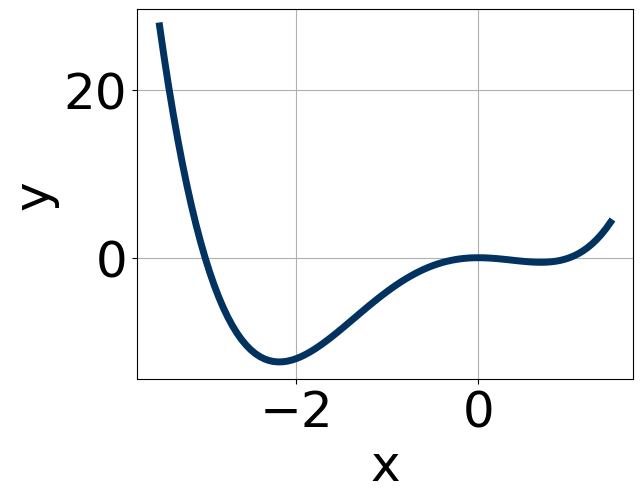
\includegraphics[width=0.5\textwidth]{../Figures/polyGraphToFunctionCopyB.png}
\end{center}




The solution is \( 7x^{6} (x - 1)^{5} (x + 3)^{9} \), which is option B.\begin{enumerate}[label=\Alph*.]
\item \( 4x^{8} (x - 1)^{6} (x + 3)^{9} \)

The factor $(x - 1)$ should have an odd power.
\item \( 7x^{6} (x - 1)^{5} (x + 3)^{9} \)

* This is the correct option.
\item \( -19x^{8} (x - 1)^{7} (x + 3)^{7} \)

This corresponds to the leading coefficient being the opposite value than it should be.
\item \( -10x^{10} (x - 1)^{11} (x + 3)^{10} \)

The factor $(x + 3)$ should have an odd power and the leading coefficient should be the opposite sign.
\item \( 9x^{11} (x - 1)^{10} (x + 3)^{9} \)

The factor $0$ should have an even power and the factor $1$ should have an odd power.
\end{enumerate}

\textbf{General Comment:} General Comments: Draw the x-axis to determine which zeros are touching (and so have even multiplicity) or cross (and have odd multiplicity).
}
\litem{
Describe the zero behavior of the zero $x = -3$ of the polynomial below.
\[ f(x) = 9(x + 3)^{3}(x - 3)^{8}(x + 2)^{4}(x - 2)^{5} \]

The solution is the graph below, which is option A.
\begin{center}
    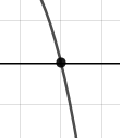
\includegraphics[width=0.3\textwidth]{../Figures/polyZeroBehaviorCopyAB.png}
\end{center}\begin{enumerate}[label=\Alph*.]
\begin{multicols}{2}
\item 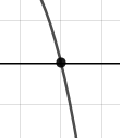
\includegraphics[width = 0.3\textwidth]{../Figures/polyZeroBehaviorCopyAB.png}
\item 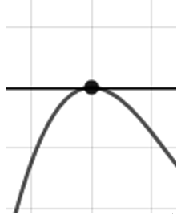
\includegraphics[width = 0.3\textwidth]{../Figures/polyZeroBehaviorCopyBB.png}
\item 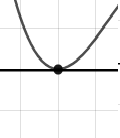
\includegraphics[width = 0.3\textwidth]{../Figures/polyZeroBehaviorCopyCB.png}
\item 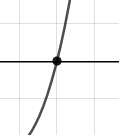
\includegraphics[width = 0.3\textwidth]{../Figures/polyZeroBehaviorCopyDB.png}
\end{multicols}\item None of the above.\end{enumerate}
\textbf{General Comment:} You will need to sketch the entire graph, then zoom in on the zero the question asks about.
}
\litem{
Which of the following equations \textit{could} be of the graph presented below?

\begin{center}
    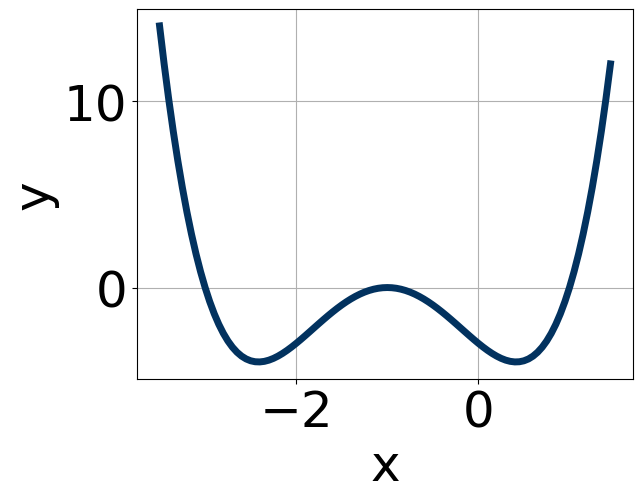
\includegraphics[width=0.5\textwidth]{../Figures/polyGraphToFunctionB.png}
\end{center}




The solution is \( 17(x + 1)^{8} (x + 3)^{11} (x - 1)^{11} \), which is option A.\begin{enumerate}[label=\Alph*.]
\item \( 17(x + 1)^{8} (x + 3)^{11} (x - 1)^{11} \)

* This is the correct option.
\item \( -18(x + 1)^{10} (x + 3)^{5} (x - 1)^{8} \)

The factor $(x - 1)$ should have an odd power and the leading coefficient should be the opposite sign.
\item \( 11(x + 1)^{8} (x + 3)^{8} (x - 1)^{11} \)

The factor $(x + 3)$ should have an odd power.
\item \( -10(x + 1)^{6} (x + 3)^{11} (x - 1)^{9} \)

This corresponds to the leading coefficient being the opposite value than it should be.
\item \( 11(x + 1)^{5} (x + 3)^{6} (x - 1)^{9} \)

The factor $-1$ should have an even power and the factor $-3$ should have an odd power.
\end{enumerate}

\textbf{General Comment:} General Comments: Draw the x-axis to determine which zeros are touching (and so have even multiplicity) or cross (and have odd multiplicity).
}
\litem{
Describe the end behavior of the polynomial below.
\[ f(x) = 7(x + 6)^{4}(x - 6)^{5}(x - 8)^{5}(x + 8)^{5} \]

The solution is the graph below, which is option D.
\begin{center}
    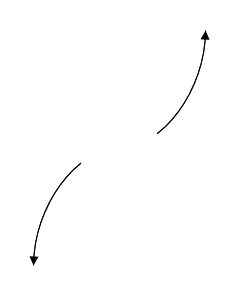
\includegraphics[width=0.3\textwidth]{../Figures/polyEndBehaviorCopyDB.png}
\end{center}\begin{enumerate}[label=\Alph*.]
\begin{multicols}{2}
\item 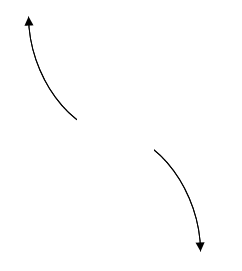
\includegraphics[width = 0.3\textwidth]{../Figures/polyEndBehaviorCopyAB.png}
\item 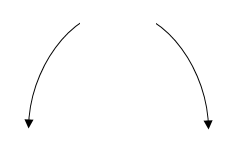
\includegraphics[width = 0.3\textwidth]{../Figures/polyEndBehaviorCopyBB.png}
\item 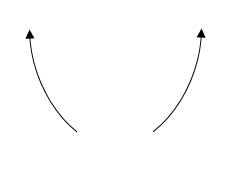
\includegraphics[width = 0.3\textwidth]{../Figures/polyEndBehaviorCopyCB.png}
\item 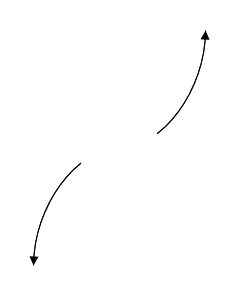
\includegraphics[width = 0.3\textwidth]{../Figures/polyEndBehaviorCopyDB.png}
\end{multicols}\item None of the above.\end{enumerate}
\textbf{General Comment:} Remember that end behavior is determined by the leading coefficient AND whether the \textbf{sum} of the multiplicities is positive or negative.
}
\litem{
Describe the end behavior of the polynomial below.
\[ f(x) = -5(x + 7)^{2}(x - 7)^{3}(x + 3)^{2}(x - 3)^{4} \]

The solution is the graph below, which is option A.
\begin{center}
    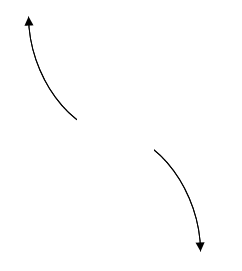
\includegraphics[width=0.3\textwidth]{../Figures/polyEndBehaviorAB.png}
\end{center}\begin{enumerate}[label=\Alph*.]
\begin{multicols}{2}
\item 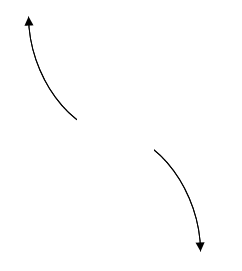
\includegraphics[width = 0.3\textwidth]{../Figures/polyEndBehaviorAB.png}
\item 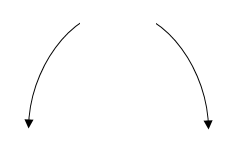
\includegraphics[width = 0.3\textwidth]{../Figures/polyEndBehaviorBB.png}
\item 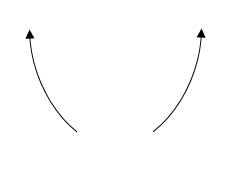
\includegraphics[width = 0.3\textwidth]{../Figures/polyEndBehaviorCB.png}
\item 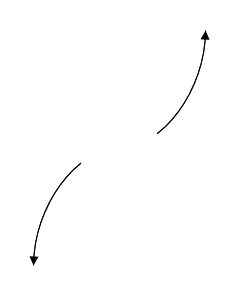
\includegraphics[width = 0.3\textwidth]{../Figures/polyEndBehaviorDB.png}
\end{multicols}\item None of the above.\end{enumerate}
\textbf{General Comment:} Remember that end behavior is determined by the leading coefficient AND whether the \textbf{sum} of the multiplicities is positive or negative.
}
\end{enumerate}

\end{document}